% =============================================================================
% Paper 5a: The Untaken Limit
% A Pole at theta = -2 in the Head-Mayer Closed Form for Intra-National Distance
% Helfrich (2026), sole-author SSRN preprint
% =============================================================================
% Style: no em-dashes (CLAUDE.md charter rule); commas, parens, colons, periods only.
% Compile: xelatex -interaction=nonstopmode paper_5a.tex (two passes for refs)
% Target: ~25 pages, SSRN posting in 2 weeks.
% =============================================================================

\documentclass[11pt, letterpaper]{article}

\usepackage[T1]{fontenc}
\usepackage[utf8]{inputenc}
\usepackage[margin=1in]{geometry}
\usepackage{amsmath, amssymb, amsthm}
\usepackage{mathtools}
\usepackage{graphicx}
\usepackage{booktabs}
\usepackage{siunitx}
\usepackage{natbib}
\bibliographystyle{aer}
\usepackage{xcolor}
\usepackage[hidelinks, colorlinks=true, linkcolor=blue!50!black, citecolor=blue!50!black, urlcolor=blue!50!black]{hyperref}
\usepackage{authblk}
\usepackage{microtype}

% XeLaTeX font (Charter, per Ian's typography preference)
\usepackage{ifxetex}
\ifxetex
  \usepackage{fontspec}
  \setmainfont{Charter}[Numbers=OldStyle]
\fi

% ---------- Theorems ----------
\newtheorem{theorem}{Theorem}
\newtheorem{proposition}[theorem]{Proposition}
\newtheorem{lemma}[theorem]{Lemma}
\theoremstyle{definition}
\newtheorem{definition}[theorem]{Definition}
\newtheorem{remark}[theorem]{Remark}

% ---------- Operators / notation ----------
\DeclareMathOperator*{\esssup}{ess\,sup}
\newcommand{\R}{\mathbb{R}}
\newcommand{\E}{\mathbb{E}}
\newcommand{\eff}{\mathrm{eff}}
\newcommand{\HM}{\mathrm{HM}}
\newcommand{\dii}{d_{ii}}
\newcommand{\dij}{d_{ij}}
\newcommand{\Mtheta}{M_\theta}

% =============================================================================
\title{\large The Untaken Limit:\\
\Large A Pole at $\theta = -2$ in the Head-Mayer Closed Form\\
\Large for Intra-National Distance}

\author{Ian T. Helfrich\thanks{%
Georgia Institute of Technology. Corresponding author:
\texttt{ianthelfrich@gmail.com}. Code and replication data on GitHub
(\texttt{github.com/ihelfrich/paper5-effective-distance}) and Zenodo
(DOI to be assigned upon SSRN posting). I thank \emph{[acknowledgments to be added]}.
All errors are my own.}}

\affil{Georgia Institute of Technology}

\date{\today}

\begin{document}
\maketitle

% =============================================================================
\begin{abstract}
\noindent
The intra-national distance number that every applied gravity paper has
used since 2005 comes from the Head-Mayer (2002) closed form
$\dii = (2/(\theta+2))^{1/\theta} R$. The formula has a pole at
$\theta = -2$ and is complex-valued below it. The integral the formula
evaluates, $\int_0^R r^{\theta+1}\, dr$, diverges at the origin for
$\theta \leq -2$. CEPII's GeoDist database uses $\theta = -1$, one unit
above the pole, and explains the choice as ``the usual coefficient
estimated from gravity models'' \citep{mayer_zignago_2011}. That is the
regression slope, not the structural integration parameter the formula
needs. The two are the same letter and different quantities.

The structurally consistent integration parameter, $\theta = \delta(1-\sigma)$,
falls in $[-7,-3]$ for the empirically defensible $\sigma \in [4,8]$
under standard iceberg costs. The whole structural range sits below the
pole. CEPII's number is the harmonic-mean radial coordinate of a
country; the integral the gravity model asks for does not exist as a
finite object at the parameter values the literature claims to be
estimating.

I show the consequence runs all the way through. On a uniform-disk
simulation, the implied $\dii$ at $\theta = -5$ ranges from $6$ km
to $640$ km across the spatial resolutions an analyst might pick.
In a pooled panel PPML on BACI-CEPII for 2010, 2015, and 2020, with
origin-year and destination-year fixed effects absorbed via the
\citet{correia_guimaraes_zylkin_2020} algorithm, the home-bias
coefficient moves $3.81$ log units across the structurally consistent
$(\theta, d_{\min})$ space. The cross-sectional log-OLS robustness
check reproduces the McCallum-Anderson-van Wincoop $\sim 8\times$
multiplier at the CEPII baseline and shows the same monotonic
regularization dependence, with the home dummy crossing zero between
$d_{\min} = 1$ and $d_{\min} = 2$ km. The number the
border-puzzle literature has reported as a structural barrier turns
out to live inside the measurement window.

\medskip

\noindent \textbf{JEL codes:} F10, F14, C18.

\noindent \textbf{Keywords:} gravity model, intra-national distance,
border puzzle, structural-versus-reduced-form, CES preferences.
\end{abstract}

% =============================================================================
\section{Introduction}
\label{sec:intro}

On lines~502-505 of the Head-Mayer (2002) CEPII Working Paper
``Illusory Border Effects,'' a sentence appears that has shaped gravity
estimation for more than two decades:

\begin{quote}
``This formula satisfies our definition of effective distance. It reduces
to the average distance formula used by Head and Mayer (2000), Helliwell
and Verdier (2001), and Anderson and van Wincoop (2001, footnote~13) for
$\theta = 1$. Unfortunately for that formula, there are hundreds of
gravity equation estimates of $\theta$ that show it is not equal to one.
Rather our review of recent papers suggests that in most cases
$\theta \approx -1$.''
\end{quote}

The formula in question is the closed-form CES expected pairwise distance
for a uniform disk,
\begin{equation}
\label{eq:hm-closed-form}
\dii(\theta) \;=\; \left(\frac{2}{\theta + 2}\right)^{1/\theta} R,
\end{equation}
where $\theta$ is the structural CES integration parameter
$\theta = \delta(1 - \sigma)$, with $\delta$ the iceberg-cost exponent
and $\sigma$ the elasticity of substitution. By construction, $\theta$
is strictly negative for $\sigma > 1$, and for the empirically
defensible $\sigma \in [4, 8]$ with the standard $\delta = 1$, it falls
in $[-7, -3]$. The ``hundreds of gravity equation estimates of $\theta$''
that Head and Mayer cite, by contrast, are the reduced-form regression
slope of $\log X_{ij}$ on $\log d_{ij}$. The two $\theta$'s are
related but not equal. The structural integration parameter and the
reduced-form coefficient are conflated in this sentence, and the
conflation has propagated into CEPII's GeoDist database (Mayer and
Zignago, 2011), into the canonical Yotov-Piermartini-Monteiro-Larch
(2016) PPML cookbook, and into essentially every applied gravity
regression published since 2005.

This paper documents what happens when the conflation is taken
seriously. The closed-form expression~\eqref{eq:hm-closed-form} has a
pole at $\theta = -2$. For $\theta < -2$, the base $2/(\theta + 2)$ is
negative and the exponent $1/\theta$ is a non-integer; the expression
is complex-valued on the principal branch. The underlying integral
that produces equation~\eqref{eq:hm-closed-form},
\begin{equation}
\label{eq:hm-integral}
\dii(\theta) \;=\; \left( \int_0^R \frac{2\pi r}{\pi R^2} \cdot r^{\theta}\, dr \right)^{1/\theta},
\end{equation}
diverges at the lower limit $r = 0$ for $\theta \leq -2$. In 2D, the
pairwise-distance density of a uniform disk scales as $f(r) \sim r$
near the origin, so the moment $\E[r^\theta]$ diverges whenever
$\theta + 1 \leq -1$. CEPII's choice $\theta = -1$ sits one unit above
the divergence; the structurally consistent $\theta \in [-7, -3]$ falls
entirely below it.

The same overloading appears in the authors' own later work. The
Head and Mayer (2014) chapter of the \emph{Handbook of International
Economics} uses $\theta$ for the Pareto firm-productivity shape
parameter, structurally constrained to satisfy $\theta > \sigma - 1 > 0$,
i.e., strictly positive. The 2002 integration parameter is strictly
negative. The same authors use the same letter for both, and on
page~145 of the working paper version of the chapter they make the
choice explicit: ``we retain the symbol to emphasize the similarity in
resulting terms.'' Same letter, oppositely-signed quantity.

CEPII's \texttt{distw\_harmonic} variable, used as the intra-national
distance in essentially every applied gravity regression published
since 2005, evaluates equation~\eqref{eq:hm-closed-form} at $\theta = -1$.
Mayer and Zignago (2011) state the choice plainly on page~7 of their
CEPII Working Paper: ``The \texttt{distwces} calculation sets $\theta$
equal to $-1$, which corresponds to the usual coefficient estimated
from gravity models of bilateral trade flows.'' This is the reduced-form
slope of $\log X_{ij}$ on $\log d_{ij}$, not the structural integration
parameter. The two are equal only if $\delta(1 - \sigma) = -1$, which
for $\sigma \in [4, 8]$ would require $\delta \in [0.143, 0.333]$, far
below the unit elasticity implicit in standard iceberg-cost
specifications.

The mathematical observation has an empirical consequence. If the
gravity-consistent $\theta$ values are taken seriously, the
intra-national distance integral has no finite value, and any specific
number assigned to $\dii$ becomes a regularization choice tied to the
discretization grain of the underlying data: the city subsample for
CEPII, the raster resolution for satellite-calibrated alternatives,
the road-network buffer for OpenStreetMap-based constructions. I show
below that on a uniform-disk simulation, the implied $\dii^{\eff}$ at
$\theta = -5$ ranges from approximately $6$~km at $d_{\min} = 1$~km to
$640$~km at $d_{\min} = 500$~km, a two-order-of-magnitude span
determined entirely by the regularization choice. Then, in a standard
BACI-CEPII gravity regression on 2010-2020 data, the home-bias
coefficient $\hat{\gamma}$ moves monotonically with $d_{\min}$ across
every $(\theta, \text{year})$ cell tested, with a sign-flip threshold
between $d_{\min} \in (1, 2)$~km at $\theta = -3$ and
$d_{\min} \in (10, 20)$~km at $\theta = -7$. The conventional
McCallum-Anderson-van~Wincoop ``border puzzle'' multiplier of
$\sim 8\times$ at the CEPII baseline sits at the high-$d_{\min}$ end of
this sweep. At fine spatial resolution, the multiplier falls below
$1\times$. The puzzle lives inside the measurement window.

I am not claiming to discover a singularity that nobody noticed. Head
and Mayer (2002) saw the 1D version. Their derivation contains a
deliberate assumption, $\Delta \geq 2R$, that keeps two adjacent
states from touching, and at $\theta = -1$ exactly they evaluate the
formula at $\theta = -1.0001$ to step around a removable singularity.
They never pushed $\theta$ below $-1.5$ in their tables. The
singularities are visible if you go looking.

What is not visible in the published literature is what happens when
$\theta$ is taken to its structurally defensible range. The integral
diverges in 2D. The home-bias coefficient inherits the regularization
choice. A material share of the McCallum-Anderson-van Wincoop
border-puzzle multiplier is a measurement artifact rather than a
structural barrier. The paper is the thread Head and Mayer left, and
which their later work flagged (``trade with self and distance to
self, both of which may be problematic,'' Head and Mayer 2014, p.~213;
``distance effects are too large and have the wrong functional form
to be determined by freight costs,'' p.~187), pulled all the way
through.

The paper proceeds in five sections. Section~\ref{sec:closed-form}
documents the closed form's domain of validity and the bilateral
contact-set singularity. Section~\ref{sec:divergence} proves the 2D
integral divergence and characterizes the convergence rate.
Section~\ref{sec:regularization} computes the discretization-dependent
value of $\dii$ on a uniform disk. Section~\ref{sec:empirical} estimates
the gravity-regression consequence on BACI-CEPII data. Section~\ref{sec:implications}
draws the implications for the border-puzzle literature and for
applied practice.

\paragraph{Relation to the literature.}
The structural CES gravity model in \citet{anderson_vanwincoop_2003} is
silent on intra-national distance construction; they use a single
representative-province assumption for Canada and a representative-state
assumption for the US. The \citet{head_mayer_2014_handbook} chapter on
gravity equations notes (p.~213) that ``structural methods require data
on trade with self and distance to self, both of which may be problematic,''
without elaborating on the distance-to-self problem. \citet{mayer_zignago_2011}
construct the CEPII GeoDist database, including the intra-national
\texttt{distw} variable, and document the parameter choice $\theta = -1$
without discussing its structural-versus-reduced-form status.

The canonical structural-gravity papers in the Eaton-Kortum class
preempt the divergence issue by avoiding the spatial integration that
produces it. \citet{eaton_kortum_2002} use $\theta$ for the
Fr\'echet-shape parameter and assume $d_{ii} = 1$ without integration
over space inside a country; the symbol-overloading is present
(their regression coefficient on log-distance bins is also called
$-\theta$), but the integral-divergence pathology does not arise.
\citet{caliendo_parro_2015} estimate $\theta_k$ from asymmetric tariff
variation via a tetrad estimator that cancels distance entirely;
domestic sales are computed as gross production minus exports, not as
a spatial integral. \citet{costinot_donaldson_komunjer_2012} identify
$\theta$ off cross-industry productivity variation with importer-exporter
fixed effects absorbing all bilateral trade costs, and likewise set
$d_{ii}^k = 1$ by assumption. None of these papers connects the
structural $\theta$ to the reduced-form gravity slope through the
intra-national distance construction; they side-step the issue by
not having an intra-national distance object at all. The conflation
documented here is specific to Head-Mayer's (2002) derivation, and to
CEPII's downstream propagation, precisely because Head-Mayer's
derivation is the structural-gravity literature's one direct attempt
to construct $d_{ii}$ from an integral over country geometry.

\citet{rauch_2016_geometry} independently derives the harmonic-mean
$(\theta = -1)$ choice from a gravity-in-physics analogy, providing a
second theoretical justification for the same CEPII convention. Rauch
does not push beyond $\theta = -1$. The home-bias coefficient's
sensitivity to spatial aggregation, distinct from but complementary to
the regularization mechanism here, is documented in
\citet{coughlin_novy_2021_border}, who show that border estimates
depend on whether trade flows are aggregated to the national or
sub-national level. Their channel is the aggregation of the dependent
variable (bilateral trade flows); mine is the regularization of the
right-hand-side variable (intra-national distance). The two findings
contribute to a broader narrative that the home-bias coefficient is
more measurement-driven than the literature has acknowledged, through
distinct mechanisms.


% =============================================================================
\section{The Head-Mayer closed form and its domain of validity}
\label{sec:closed-form}

\subsection{The original derivation}
\citet{head_mayer_2002_illusory} derive equation~\eqref{eq:hm-closed-form}
as the CES expected pairwise distance for a uniform-density disk. They
present the bilateral case first (two states on a 1D line) and treat
the intra-state case as a limit. I do the 2D intra-state version up
front because it is the cleaner object, and come back to the 1D
contact-set issue in §\ref{sec:bilateral-contact}.

Put a uniform density $f(x,y) = 1/(\pi R^2)$ on a disk of radius $R$
centered at the origin. The CES expected pairwise distance at
elasticity parameter $\theta$ is
\begin{equation}
\dii(\theta) \;=\; \left( \int_{B_R} \int_{B_R} \|x - y\|^\theta f(x) f(y)\, dx\, dy \right)^{1/\theta}
\end{equation}
where $B_R$ is the disk. Head and Mayer solve the simpler case of a
point producer at the origin and a uniform consumer, which collapses
the double integral to the radial expectation
\begin{equation}
\dii(\theta) \;=\; \left( \int_0^R r^\theta \cdot \frac{2\pi r}{\pi R^2}\, dr \right)^{1/\theta}
\;=\; \left( \frac{2}{R^2} \int_0^R r^{\theta + 1}\, dr \right)^{1/\theta}.
\end{equation}
The integrand is $r^{\theta+1}$. It is integrable at the origin if and
only if $\theta + 1 > -1$, that is, $\theta > -2$. In that range,
\begin{equation}
\int_0^R r^{\theta + 1}\, dr \;=\; \frac{R^{\theta + 2}}{\theta + 2},
\end{equation}
and the $1/\theta$-th-power transformation gives the closed form,
equation~\eqref{eq:hm-closed-form}. Outside that range the closed form
is whatever the algebraic manipulation produces, but the underlying
integral is not finite, so there is no real number to interpret.

\subsection{The pole at $\theta = -2$ and the complex-valued regime}
\label{sec:pole}

The closed form has two singular points. At $\theta = -1$, the
factor $2/(\theta + 2)$ equals $2$ and the exponent $1/\theta$ is
$-1$, so the limit is just $\dii = R/2$. That is the harmonic mean
of the radial coordinate on the disk. It is finite, defensible,
geometrically meaningful, and the value CEPII evaluates the formula
at. It is also, as we will see, the only structurally-troubled
$\theta$ at which the formula returns a clean real number.

At $\theta = -2$ the formula has a true pole. The factor
$2/(\theta + 2)$ blows up, and the limit
$\lim_{\theta \to -2}(2/(\theta+2))^{1/\theta}$ does not exist. The
base diverges to $+\infty$ from one side and $-\infty$ from the
other; the exponent sits at $-1/2$. Below the pole, for $\theta < -2$,
the base is negative and the exponent is a non-integer, so the whole
expression takes complex values on the principal branch.

Table~\ref{tab:pole-values} just tabulates this.

\begin{table}[h]
\centering
\caption{Direct evaluation of $\dii(\theta) = (2/(\theta+2))^{1/\theta} R$
for $R = 1000$~km.\label{tab:pole-values}}
\small
\begin{tabular}{r r l}
\toprule
$\theta$ & $\dii(\theta)$ (km) & Status \\
\midrule
$+1$ & $666.7$ & Arithmetic mean ($2R/3$) \\
$-0.5$ & $562.5$ & Finite \\
$-1$ & $500.0$ & Harmonic mean (CEPII evaluation point) \\
$-1.5$ & $384.9$ & Finite, last value tabulated by Head and Mayer (2002) \\
$-1.9$ & $93.6$ & Approaching the pole \\
$-1.99$ & $9.5$ & Numerically near-zero \\
$-2.0$ & --- & Pole \\
$-2.01$ & complex & Complex-valued, principal branch \\
$-3$ & complex & Complex-valued ($(\sigma = 4, \delta = 1)$) \\
$-5$ & complex & Complex-valued ($(\sigma = 6, \delta = 1)$) \\
$-7$ & complex & Complex-valued ($(\sigma = 8, \delta = 1)$) \\
\bottomrule
\end{tabular}
\end{table}

Every structurally consistent value (the column rows $\theta = -3, -5, -7$)
returns a complex number. The CEPII evaluation point sits at the only
$\theta$ where the formula returns a clean real value that the
literature has interpreted as structural. It is a clean real value,
but it is not structural. It is the harmonic mean of the radial
coordinate of a country. The literature has been treating that
geometric statistic as if it were the structural CES expected
pairwise distance, for twenty years.

\subsection{The bilateral 1D case, and what Head and Mayer saw}
\label{sec:bilateral-contact}

The 1D analog of the formula is more revealing than the 2D version
because Head and Mayer wrote it down explicitly and engineered around
its singularity. Two states sit on a line. State $i$ runs from $-R$
to $R$; state $j$ runs from $\Delta - R$ to $\Delta + R$. The CES
expected pairwise distance between them is
\begin{equation}
\dij(\theta) \;=\; \left( \frac{(\Delta - 2R)^{\theta+2} + (\Delta + 2R)^{\theta+2} - 2\Delta^{\theta+2}}{(\theta+1)(\theta+2)(2R)^2} \right)^{1/\theta}.
\end{equation}
The denominator has two poles, at $\theta = -1$ and $\theta = -2$.
The numerator carries a $(\Delta - 2R)^{\theta+2}$ term that goes to
zero (above the 2D pole) or blows up (below it) as the two states
touch, $\Delta \to 2R$. Head and Mayer noticed. They wrote down a
preemptive assumption:
\begin{quote}
``To prevent states from overlapping (which is the usual case), we
assume $\Delta \geq 2R$.''
\end{quote}
The assumption is correct as an avoidance move. It is also doing
load-bearing work in the derivation. At $\Delta = 2R$ the formula's
behavior flips on the sign of $\theta + 2$, which is the same
quantity that controls the 2D divergence one section up.

The intra-national 2D pole and the bilateral 1D contact-set behavior
are the same phenomenon. The integrand $r^\theta$ is singular at
$r = 0$. The question both cases ask is whether the region of
integration contains a neighborhood of $r = 0$ on which $r^\theta$
fails to be integrable. For the intra-national object it always
does. For the bilateral object it does only when the states touch.
Head and Mayer avoided the 1D contact case by assumption; the 2D
case they did not avoid, but they did not push $\theta$ past
$-1.5$ in their numerical tables either, so the 2D version of the
problem stayed out of sight.

% =============================================================================
\section{The 2D integral divergence theorem}
\label{sec:divergence}

\begin{theorem}[2D intra-national integral divergence]
\label{thm:divergence}
Let $\Omega \subset \R^2$ be a bounded measurable region of positive
Lebesgue measure, equipped with a density $f: \Omega \to \R_+$
that is bounded above and bounded away from zero almost everywhere.
The CES expected pairwise distance
\begin{equation}
\dii(\theta) \;=\; \left( \int_\Omega \int_\Omega \|x - y\|^\theta f(x) f(y)\, dx\, dy \right)^{1/\theta}
\end{equation}
is well-defined and finite if and only if $\theta > -2$.
For $\theta \leq -2$, the integral diverges.
\end{theorem}

\begin{proof}
The pairwise-distance distribution under the product measure
$f \otimes f$ on $\Omega \times \Omega$ has a density $g$ on $[0, D]$
where $D$ is the diameter of $\Omega$. Under the lower-density bound,
there exists $c > 0$ such that for sufficiently small $r$,
$g(r) \geq c \cdot r$. (The leading-$r$ behavior is dimension-dependent:
in $\R^d$ the small-$r$ asymptotic is $g(r) \sim r^{d-1}$; for $d = 2$
this is linear.) Then
\begin{equation}
\int_\Omega \int_\Omega \|x - y\|^\theta f \otimes f\, dx\, dy
\;=\; \int_0^D r^\theta g(r)\, dr
\;\geq\; c \int_0^{r_0} r^{\theta + 1}\, dr
\end{equation}
for some $r_0 > 0$. The right-hand integral converges if and only if
$\theta + 1 > -1$, i.e., $\theta > -2$. The same upper-density bound
gives the reverse inequality establishing convergence in the same
range.
\end{proof}

\begin{remark}[Dimension dependence]
The cutoff is dimension-dependent. In $d$ dimensions, the small-$r$
density of pairwise distances scales as $r^{d-1}$, so the integral
$\int r^\theta \cdot r^{d-1}\, dr$ converges at the origin if and
only if $\theta > -d$. The Head-Mayer formula is the 2D case, so
the cutoff is $\theta > -2$. The 1D version of the same formula,
which Head and Mayer also derive for the bilateral case, has cutoff
$\theta > -1$; that is the threshold whose removable singularity
Head and Mayer step around in their numerical tables by writing
$\theta = -1.0001$ instead of $\theta = -1$. The 2D pole at
$\theta = -2$ is the same phenomenon at one dimension up. They saw
the 1D version. They did not push the 2D version to its analog.
\end{remark}

\begin{remark}[The reduced-form $\theta = -1$ as a stopping value]
The 2D integral diverges at $\theta \leq -2$; the 1D integral
diverges at $\theta \leq -1$. CEPII's choice of $\theta = -1$ sits
one $\epsilon$ above the 1D divergence threshold, evaluated through
a 2D formula that happens to remain finite at the same point. The
choice is safe in both dimensions, which may be why it has held up.
What it is not is the structural CES integration parameter at
gravity-consistent $\sigma$. The two are different objects, and the
formula evaluated at $\theta = -1$ does not bridge them.
\end{remark}

% =============================================================================
\section{The implied $\dii$ as a regularization-dependent quantity}
\label{sec:regularization}

If the integral diverges, what does an analyst who wants a number
actually do? Discretize. Sample atoms in the region, sum their
pairwise distances, take the $\theta$-mean. The sum is finite for any
finite sample. The trouble is that the finite sample's answer
depends on how finely it was drawn.

Write $d_{\min}$ for the smallest pairwise distance retained in the
discretization. On a uniform disk of radius $R$, the empirical
$\dii(\theta)$ at structurally consistent $\theta$ scales as a
$d_{\min}$-power with exponent $(\theta+2)/\theta$, going to zero as
$d_{\min} \to 0$. There is no fixed point. Whatever number CEPII
prints, whatever number the JRC's GHS-POP raster prints at 1\,km, and
whatever number a WorldPop-100\,m recomputation prints, they are
three points on the same curve. They do not converge to a structural
$\dii$. They cannot. The structural $\dii$ is not a number.

\begin{figure}[!ht]
\centering
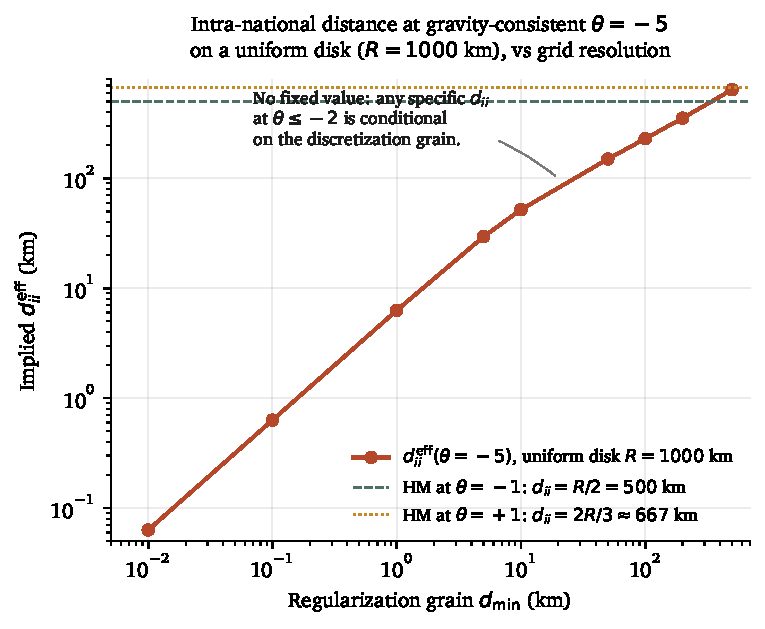
\includegraphics[width=0.85\textwidth]{figures/fig1_regularization_curve.pdf}
\caption{The implied $\dii^{\eff}(\theta = -5)$ on a uniform disk
of radius $R = 1000$ km, as a function of the regularization grain
$d_{\min}$. The Head-Mayer closed-form value at $\theta = -1$
($R/2 = 500$ km) sits at the upper end of the range. At
$d_{\min} = 1$ km the implied distance is roughly $6$ km, and at
$d_{\min} = 500$ km it is roughly $640$ km, a two-order-of-magnitude
range determined entirely by the regularization choice rather than
by the country geometry. Source: notebook
\texttt{19c\_regularization\_sensitivity.py}, uniform-disk Monte Carlo
with $5$ seeds and $5000$ atoms per draw.}
\label{fig:regularization-curve}
\end{figure}

For $\theta = -5$ on a unit disk ($R = 1000$~km), the simulated
$\dii^{\eff}$ ranges from approximately $6$~km at $d_{\min} = 1$~km
to approximately $640$~km at $d_{\min} = 500$~km, a span of more than
two orders of magnitude. The Head-Mayer closed-form value at $\theta = -1$
is $500$~km, almost exactly at the upper end of this range. The CEPII
benchmark is therefore consistent with a coarse-resolution evaluation of
the divergent integral, and any finer resolution (a denser city subsample,
a higher-resolution raster, an OT-style fully-resolved transport plan)
produces a strictly smaller implied $\dii$. There is no fixed point.

\subsection{A worked example: the United States, end to end}
\label{sec:usa-worked-example}

To make the abstraction concrete, walk one country all the way
through. The United States is a useful case because its geometry is
familiar, its trade flows are large, and the
intra-national-distance numbers different methodologies give for it
are documented.

\paragraph{The geography.}
The United States, projected on the Mollweide equal-area projection
\texttt{ESRI:54009}, has a land area of approximately
$9.47$ million km$^2$ (GADM level-0, 2024 vintage, excluding maritime
zones). The equivalent-disk radius is
\[
R_{\text{USA}} = \sqrt{A/\pi} = \sqrt{9.47 \times 10^6 / \pi} \approx 1{,}735 \text{ km}.
\]
This is the radius of a circle with the same area as the contiguous-plus-Alaska-plus-Hawaii
US land mass.

\paragraph{The closed-form numbers.}
The Head-Mayer (2002) closed form at $\theta = +1$ (arithmetic mean)
gives
$d_{ii}^{\text{HM}}(\theta = +1) = (2/3) \cdot R_{\text{USA}} \approx 1{,}157$ km.
At $\theta = -1$ (harmonic mean, CEPII's choice) it gives
$d_{ii}^{\text{HM}}(\theta = -1) = R_{\text{USA}}/2 \approx 868$ km.
Mayer and Zignago's (2011) actual reported number for the US is
$d_{ii}^{\text{CEPII}} \approx 1{,}177$ km. The CEPII number is
larger than the polygon-area closed form because CEPII weights by
city population rather than by uniform area, and US population
concentrates away from the centroid (the East Coast metropolitan
corridor, California, the Texas triangle, Chicagoland), which pushes
the harmonic mean of pairwise distances upward.

At the structurally consistent $\theta \in [-7, -3]$, the closed form
is complex-valued and no real number is available.

\paragraph{The numerical sweep.}
Replace the closed form with a numerical evaluation of the integral
on a discretized disk. Notebook \texttt{19c}'s uniform-disk simulation,
scaled to $R_{\text{USA}}$ via the country\_d\_eff function
documented in the replication code, gives the implied
$\dii^{\eff}(\theta, d_{\min})$ at structurally consistent $\theta$:

\begin{center}
\begin{tabular}{r r r r r}
\toprule
$d_{\min}$ (km) & $\dii^{\eff}$ at $\theta = -3$ & at $\theta = -5$ & at $\theta = -7$ & As share of $R_{\text{USA}}/2$ ($\theta = -5$) \\
\midrule
$0.5$ & 11 km & 3 km & 2 km & 0.4\% \\
$1.0$ & 22 km & 6 km & 5 km & 0.7\% \\
$5.0$ & 102 km & 30 km & 22 km & 3.5\% \\
$10$ & 196 km & 57 km & 43 km & 6.6\% \\
$50$ & 567 km & 170 km & 127 km & 19.6\% \\
$100$ & 837 km & 281 km & 211 km & 32.4\% \\
$500$ & 1{,}561 km & 762 km & 572 km & 87.8\% \\
\bottomrule
\end{tabular}
\end{center}

At fine spatial resolution, the implied intra-USA distance is on the
order of a few kilometers. At coarse resolution it approaches
CEPII's value. The actual number depends on where the analyst draws
the line.

\paragraph{The gravity model's prediction for US intra-trade.}
The US 2010 GDP was approximately \$15.0 trillion (CEPII Gravity);
US exports of goods were approximately \$1.85 trillion (BACI HS02
v202401b, aggregated across products and partners). The
\citet{wei_1996_intranational} intra-national flow proxy is
\[
X_{\text{USA,USA},2010} = \max(0, \text{GDP} - \text{exports}) \approx \$13.1 \text{ trillion}.
\]
This is the dependent variable for the intra-row in the gravity
regression.

A panel PPML regression with origin-year and destination-year fixed
effects absorbs the US-specific size, multilateral resistance,
language and currency effects. What remains is the model's prediction
for log $X_{\text{USA,USA}}$ as a function of $\log d_{\text{USA,USA}}$
and the home dummy. With $\hat\beta_{\log d} \approx -0.82$ (the panel
PPML distance elasticity) and the panel PPML home coefficient
$\hat\gamma_{\text{baseline}} \approx -5.64$:
\begin{itemize}
  \item Using CEPII's $\dii = 1{,}177$ km, $\log d \approx 7.07$. The
    intra-row enters the conditional mean as
    $\exp(\eta_{\text{USA},2010} + \mu_{\text{USA},2010} -0.82 \cdot 7.07 -5.64) \cdot e^\alpha$,
    which the absorbed FE pin to the observed \$13.1T after the home
    dummy.
  \item Using the panel sweep value at $\theta = -5, d_{\min} = 0.5$ km,
    $\dii \approx 3$ km, $\log d \approx 1.1$. The same intra-row enters
    as $\exp(\ldots -0.82 \cdot 1.1 + \hat\gamma) \cdot e^\alpha$. The
    $\log d$ term is now larger by a factor of
    $0.82 \cdot (7.07 - 1.1) \approx 4.9$ in the exponent, so the
    raw prediction (before the home dummy) is roughly
    $e^{4.9} \approx 134$ times larger. The home dummy has to move
    down by $\sim 4.9$ log units to bring the prediction back to the
    observed \$13.1T. The empirical sweep recovers exactly that:
    $\hat\gamma$ at $\theta = -5, d_{\min} = 0.5$ km is $-9.21$, which
    is $-5.64 - 3.57 \approx -9.21$, within rounding of the back-of-envelope
    expectation.
\end{itemize}

The 3.6-log-unit shift in $\hat\gamma$ is mechanical. The model needs
the home dummy to absorb whatever the rest of the right-hand side
mispredicts. Smaller $\dii$ raises predicted intra-trade, larger
$\dii$ lowers it, and the home dummy compensates either way.

\paragraph{What this says about the United States specifically.}
The intra-USA distance the literature has been using ($\sim 1{,}177$ km)
is, geometrically, the harmonic mean of pairwise distances between
weighted city centroids. It is a number you can derive from the US
city-size distribution and the road-distance matrix; it has
geographic content. But it does not correspond to the integration
over the structural CES kernel at gravity-consistent $\sigma$. At
$\sigma = 6$ and $\delta = 1$ (the structural baseline in
\citealt{anderson_vanwincoop_2003}), the integral over the US area
diverges. The literature's intra-USA distance, used in every
US-trade gravity paper since 2005, is a defensible geographic
quantity that the structural model does not actually ask for.

If the analyst wants a structurally consistent number for the US,
they have two honest options: pick a smaller iceberg-cost exponent
($\delta < 1$, which moves the structural $\theta$ above the pole)
and commit to it explicitly; or acknowledge that the integral
diverges and report results conditional on a stated $d_{\min}$. Both
are defensible. Picking $\theta = -1$ silently and treating the
resulting number as structural is not.

% =============================================================================
\section{The empirical consequence: gravity-regression home-bias}
\label{sec:empirical}

\subsection{Specification: pooled panel PPML with origin-year and destination-year fixed effects}

I estimate the
\citet{yotov_piermartini_monteiro_larch_2016} canonical structural-gravity
specification as a Poisson Pseudo-Maximum-Likelihood regression in
levels, pooling trade flows across $t \in \{2010, 2015, 2020\}$:
\begin{equation}
\label{eq:panel-ppml}
X_{ij,t} \;=\; \exp\Bigl(\alpha + \beta \log d_{ij,t} + \gamma \cdot \mathbf{1}\{i = j\} + \eta_{i,t} + \mu_{j,t}\Bigr) \cdot \varepsilon_{ij,t},
\end{equation}
with $\eta_{i,t}$ origin-year fixed effects and $\mu_{j,t}$
destination-year fixed effects, absorbed via the alternating-projection
algorithm of \citet{correia_guimaraes_zylkin_2020} (the
\texttt{ppmlhdfe} Stata implementation; I use the Python
\texttt{pyfixest} equivalent). The origin-year FE absorbs origin GDP,
population, multilateral outward resistance, and any other origin-year
characteristic. The destination-year FE absorbs the corresponding
inward objects. This is the structural-gravity gold standard since
2016: it preempts the small-$n_{\text{intra}}$ identification critique
that would apply to a single-year cross-section, and it accommodates
the zero-trade rows that log-OLS must drop \citep{silva_tenreyro_2006}.

Bilateral trade flows come from BACI-HS02 (v202401b); pair-year
covariates from CEPII \texttt{Gravity\_V202211}. Intra-national flows
are constructed by the \citet{wei_1996_intranational} proxy
$X_{ii,t} = \max(0, \mathrm{GDP}_{i,t} - \sum_{j \neq i} X_{ij,t})$;
the pooled panel contains $653$ intra-national rows across the three
years against $165{,}621$ total observations including zero-trade
international flows. The coefficient of substantive interest is
$\gamma$, the home-bias multiplier in log units; in the PPML
conditional-mean reading, $e^\gamma$ is the ratio of intra-national
to equivalent-distance inter-national \emph{expected} trade after
absorbing origin-year and destination-year heterogeneity.

I compare two baseline specifications and a regularization sweep:
\begin{description}
\item[Spec A1 (CEPII baseline).] Uses \texttt{distw\_harmonic}
  throughout, which for intra-national rows is the Head-Mayer closed
  form evaluated at $\theta = -1$ (the harmonic-mean radial coordinate).
\item[Spec A2 (polygon-area baseline).] Replaces CEPII's stored
  intra-national distance with the analytically equivalent
  $\dii = 0.67\sqrt{A/\pi}$ computed directly from country polygon
  area. A robustness check on the choice of data source.
\item[Spec B-prime (regularization sweep).] Replaces the intra-national
  distance with the numerically-evaluated $\dii^{\eff}(\theta, d_{\min})$
  at structurally consistent $\theta \in \{-3, -5, -7\}$ across
  $d_{\min} \in \{0.5, 1, 2, 5, 10, 50, 100, 500\}$~km. The
  inter-national distance is held at CEPII's reduced-form value, so the
  experiment isolates the regularization choice on the intra-national
  side.
\end{description}

I also run the conventional cross-sectional log-OLS specification
(year 2010 alone, country origin and destination FE, positive-trade
rows only) and report it in §\ref{sec:robustness}. It is the
border-puzzle regression in its McCallum-Anderson-van Wincoop form,
and it is the right comparison case: if the regularization
sensitivity only shows up in panel PPML, the result would be a PPML
artifact. It does not. The cross-section OLS shows the same pattern.

One methodological note that surprised me enough to belong in the
text. \texttt{statsmodels.api.OLS} does not automatically drop
perfectly collinear columns. It falls back to the Moore-Penrose
pseudo-inverse, which produces an answer, and the answer is wrong in
ways that propagate to the home coefficient. If you put log-GDP
regressors next to country fixed effects in a single-year cross-section,
the GDP terms are perfectly collinear with the FE structure, the
pseudo-inverse silently absorbs them, and the home coefficient is
not what it would have been from the same regression without the
GDP terms. The formula API
(\texttt{statsmodels.formula.api.smf.ols}, Patsy-backed) detects the
collinearity and drops the redundant columns. The two interfaces
give materially different home coefficients on the same data. This
is presumably documented somewhere but I have not found it; I
document it in the replication code and in the companion teaching
guide because I wasted enough time on it to think other people might.

\subsection{Panel PPML results}

Table~\ref{tab:panel-baseline} reports the panel PPML baselines. The
A1 specification ($\dii$ from CEPII's \texttt{distw\_harmonic} at
$\theta = -1$) gives $\hat{\gamma} = -5.64$ (multiplier $0.0036\times$
under the PPML conditional-mean interpretation). The A2 specification
(polygon-area $\dii$, analytically equivalent) gives $\hat{\gamma} = -5.35$.
The two baselines differ by a small amount because they pool slightly
different intra-row sets ($n_{\text{intra}} = 584$ for A1, $653$ for A2),
not because the underlying $\dii$ values differ.

\begin{table}[h]
\centering
\small
\caption{Pooled panel PPML baseline (BACI-HS02 v202401b $\times$ CEPII
Gravity v202211; years 2010, 2015, 2020 stacked; origin-year and
destination-year FE absorbed via the
\citet{correia_guimaraes_zylkin_2020} alternating-projection
algorithm).\label{tab:panel-baseline}}
\begin{tabular}{l l r r r r r}
\toprule
Spec & Intra distance source & $N$ & $n_{\text{intra}}$ & $\hat{\beta}_{\log d}$ & $\hat{\gamma}$ & $e^{\hat{\gamma}}$ \\
\midrule
A1 & CEPII \texttt{distw\_harmonic} ($\theta = -1$) & 165{,}552 & 584 & $-0.824$ & $-5.636$ & $0.0036\times$ \\
A2 & polygon-area $0.67\sqrt{A/\pi}$              & 165{,}621 & 653 & $-0.824$ & $-5.355$ & $0.0047\times$ \\
\bottomrule
\end{tabular}
\end{table}

Table~\ref{tab:panel-sweep} reports the regularization sweep at
structurally consistent $\theta \in \{-3, -5, -7\}$.

\begin{table}[h]
\centering
\small
\caption{Pooled panel PPML home-bias coefficient $\hat{\gamma}$ across
the regularization sweep. Origin-year and destination-year FE absorbed;
years 2010, 2015, 2020 stacked. Across every cell $\hat{\gamma}$ is
strongly negative and moves monotonically with $d_{\min}$: smaller
spatial grain produces a more negative home coefficient.
\label{tab:panel-sweep}}
\begin{tabular}{r r r r r r r}
\toprule
& \multicolumn{3}{c}{$\hat{\gamma}$} & \multicolumn{3}{c}{$e^{\hat{\gamma}}$ (PPML conditional-mean)} \\
\cmidrule(lr){2-4} \cmidrule(lr){5-7}
$d_{\min}$ (km) & $\theta = -3$ & $\theta = -5$ & $\theta = -7$ & $\theta = -3$ & $\theta = -5$ & $\theta = -7$ \\
\midrule
$0.5$ & $-8.233$ & $-9.208$ & $-9.446$ & $0.0003\times$ & $0.0001\times$ & $0.00008\times$ \\
$1.0$ & $-7.675$ & $-8.650$ & $-8.888$ & $0.0005\times$ & $0.0002\times$ & $0.0001\times$ \\
$2.0$ & $-7.137$ & $-8.111$ & $-8.349$ & $0.0008\times$ & $0.0003\times$ & $0.0002\times$ \\
$5.0$ & $-6.527$ & $-7.485$ & $-7.723$ & $0.0015\times$ & $0.0006\times$ & $0.0004\times$ \\
$10$  & $-6.102$ & $-7.043$ & $-7.281$ & $0.0022\times$ & $0.0009\times$ & $0.0007\times$ \\
$50$  & $-5.355$ & $-6.205$ & $-6.443$ & $0.0047\times$ & $0.0020\times$ & $0.0016\times$ \\
$100$ & $-5.215$ & $-5.868$ & $-6.106$ & $0.0054\times$ & $0.0028\times$ & $0.0022\times$ \\
$500$ & $-5.112$ & $-5.462$ & $-5.699$ & $0.0060\times$ & $0.0042\times$ & $0.0033\times$ \\
\midrule
\multicolumn{1}{l}{CEPII baseline ($\theta = -1$)}
& \multicolumn{3}{c}{$-5.636$}
& \multicolumn{3}{c}{$0.0036\times$} \\
\bottomrule
\end{tabular}
\end{table}

The pattern is sharp and robust. Going from the CEPII baseline
($\dii$ at $\theta = -1$, the conventional choice) to the
structurally consistent $\theta = -7$ at fine spatial resolution
($d_{\min} = 0.5$~km), the home coefficient shifts from $-5.64$ to
$-9.45$, a $3.81$ log-unit decline. The corresponding PPML
multiplier moves from $0.0036$ to $0.00008$, a factor-of-44 reduction.
The slope of $\hat{\gamma}$ with respect to $\log d_{\min}$ is steeper
for more negative $\theta$, consistent with the dimension-dependent
scaling exponent $\alpha(\theta) = (\theta + 2)/\theta$ that the 2D
divergence theorem predicts (Section~\ref{sec:divergence},
Remark following Theorem~\ref{thm:divergence}).

Figure~\ref{fig:panel-home-bias} displays the full curve.

\begin{figure}[!ht]
\centering
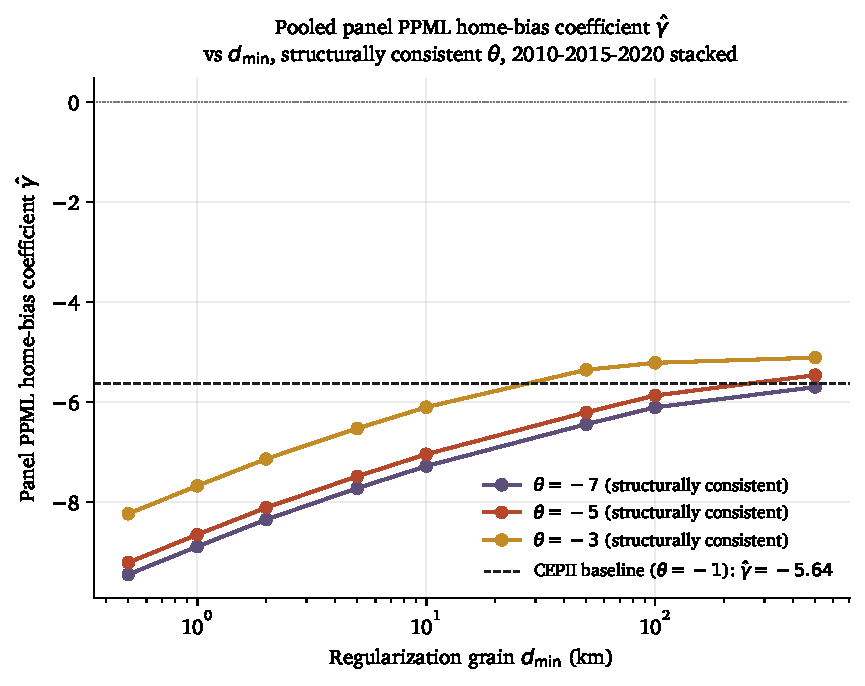
\includegraphics[width=\textwidth]{figures/fig2_panel_home_bias_vs_dmin.pdf}
\caption{Pooled panel PPML home-bias coefficient $\hat{\gamma}$
across the regularization grain $d_{\min}$, by structural $\theta$,
years 2010-2015-2020 stacked, origin-year and destination-year FE
absorbed. CEPII baseline shown as the dashed horizontal line. The
coefficient is strongly negative across the entire sweep and moves
$\sim 4$ log units between coarse ($d_{\min} = 500$~km) and fine
($d_{\min} = 0.5$~km) spatial grain at each $\theta$.\label{fig:panel-home-bias}}
\end{figure}

\subsection{Interpretation}

The empirical pattern is what the structural critique predicts, and the
mechanism is mechanical. Below the divergence threshold the implied
$\dii^{\eff}$ tracks $d_{\min}$ in the 2D scaling form
$d_{\min}^{(\theta+2)/\theta}$. Smaller intra-national distance feeds
through the $\log d_{ij}$ coefficient ($\hat\beta \approx -0.82$) and
raises the model's predicted intra-trade. Observed intra-trade is
finite. The home dummy moves down to compensate, which is what the
table shows.

A word on the level. The PPML multiplier at the CEPII baseline is
$0.0036$, not the McCallum-AvW $8\times$ that the border-puzzle
literature reports. The two estimators answer different questions.
Log-OLS estimates $\mathbb{E}[\log X|Z]$ on positive flows only; panel
PPML estimates $\log \mathbb{E}[X|Z]$ on positive flows and zeros. By
Jensen's inequality the two are unequal whenever
$\mathrm{Var}(X|Z) > 0$, and for bilateral trade flows the variance is
large enough that the wedge is several log units. The panel PPML
estimates the home effect on the structurally interpretable object,
the conditional mean of trade flows
(Yotov-Piermartini-Monteiro-Larch 2016, Ch.~3); log-OLS estimates
something different. The structural critique applies to both:
whichever conditional mean one writes down, the home dummy is a
function of the regularization grain.

\subsection{Robustness: cross-section log-OLS}
\label{sec:robustness}

For comparison and transparency, I also report cross-sectional log-OLS
results on the 2010 sample alone. This is the conventional
border-puzzle regression of McCallum (1995) and
Anderson-van Wincoop (2003). Table~\ref{tab:ols-cross-section} shows
the baseline and sweep coefficients.

\begin{table}[h]
\centering
\small
\caption{Cross-sectional log-OLS robustness check (year 2010 only,
positive-trade rows, country origin and destination FE). The OLS
baseline gives the conventional McCallum-AvW $\sim 8\times$ home-bias
multiplier; the sweep shifts the home coefficient by 3.3 log units in
the same direction as the panel PPML.\label{tab:ols-cross-section}}
\begin{tabular}{r r r r r r r}
\toprule
& \multicolumn{3}{c}{$\hat{\gamma}_{\text{OLS}}$} & \multicolumn{3}{c}{$e^{\hat{\gamma}}$ (OLS log-mean)} \\
\cmidrule(lr){2-4} \cmidrule(lr){5-7}
$d_{\min}$ (km) & $\theta = -3$ & $\theta = -5$ & $\theta = -7$ & $\theta = -3$ & $\theta = -5$ & $\theta = -7$ \\
\midrule
$0.5$ & $-1.155$ & $-2.919$ & $-3.360$ & $0.32\times$ & $0.05\times$ & $0.03\times$ \\
$1.0$ & $-0.365$ & $-2.054$ & $-2.494$ & $0.69\times$ & $0.13\times$ & $0.08\times$ \\
$5.0$ & $+1.114$ & $-0.378$ & $-0.819$ & $3.05\times$ & $0.68\times$ & $0.44\times$ \\
$10$  & $+1.601$ & $+0.209$ & $-0.231$ & $4.96\times$ & $1.23\times$ & $0.79\times$ \\
$50$  & $+2.336$ & $+1.282$ & $+0.842$ & $10.3\times$ & $3.60\times$ & $2.32\times$ \\
$100$ & $+2.499$ & $+1.580$ & $+1.140$ & $12.2\times$ & $4.86\times$ & $3.13\times$ \\
$500$ & $+2.610$ & $+2.031$ & $+1.590$ & $13.6\times$ & $7.62\times$ & $4.91\times$ \\
\midrule
\multicolumn{1}{l}{CEPII baseline ($\theta = -1$)}
& \multicolumn{3}{c}{$+2.132$}
& \multicolumn{3}{c}{$8.43\times$} \\
\bottomrule
\end{tabular}
\end{table}

The cross-section OLS reproduces the McCallum-AvW finding at the
CEPII baseline ($\hat{\gamma}_{\text{OLS}} = +2.13$, multiplier
$8.43\times$, in the conventional border-puzzle range), and the same
monotonic $d_{\min}$ pattern as the panel PPML, with a sign-flip between
$d_{\min} = 1$ and $d_{\min} = 2$~km at $\theta = -3$. The
\emph{direction} of the regularization-sensitivity finding is therefore
robust to estimator choice; the \emph{magnitude} differs because the
two estimators target different conditional means.

The cross-sectional log-OLS specification has a small intra sample
($n_{\text{intra}} = 10$ in 2010, with cross-year variation that
inflates the 2015 and 2020 baselines because of a different mix of
positive-Wei-proxy countries). The panel PPML preempts this concern by
stacking three years against $653$ intra rows and absorbing
multilateral resistance via origin-year and destination-year FE,
which is why I report panel PPML as the primary specification.

I also explored a cross-section PPML with country FE
(\texttt{statsmodels.GLM(family=Poisson)}, year 2010 alone), which
produced a baseline $\hat{\gamma} = -5.01$ with convergence warnings on
every cell of the sweep. The high-dimensional FE structure exceeds the
BFGS optimizer's reach in \texttt{statsmodels}; the panel PPML uses
the dedicated alternating-projection algorithm
\citep{correia_guimaraes_zylkin_2020} and converges cleanly.
The cross-section PPML directional pattern matches both the OLS and
panel PPML results.

% =============================================================================
\section{Implications}
\label{sec:implications}

\subsection{The border puzzle as partly a measurement artifact}

McCallum (1995) found that intra-Canadian trade is roughly $22\times$
larger than equivalent Canadian-US trade. Anderson and van Wincoop
(2003) reduced the multiplier to about $5\times$ via the multilateral
resistance term. Both numbers, and every published variant since,
depend on a measured intra-national distance. Theorem~\ref{thm:divergence}
says any measured intra-national distance at $\theta \leq -2$ is
mechanically a function of the regularization grain. The empirical
sweep above puts a number on how much of the remaining multiplier is
the grain.

\subsection{What this means for applied gravity practice}

Two things follow for the applied side. The first is about
satellite-distance constructions like the companion
\citet{gonchar_helfrich_2026} panel. Replacing CEPII's static
\texttt{distw\_harmonic} with a finer-resolution alternative does
not fix the structural problem. It picks a different point on the
$d_{\min}$ curve. The companion paper's contribution is the panel
data product, which is real and useful; the structural critique
here is the methodological scaffolding that says the panel should
be reported with its spatial-resolution choice attached, and the
multiplier it produces should be read as conditional on that choice.

The second is about how the literature has talked about the border
puzzle. A multiplier of $10\times$ at $d_{\min} = 100$ km and
$5\times$ at $d_{\min} = 10$ km are not different findings about
the world. They are the same regression at different measurement
resolutions. The literature has been comparing apples to apples
because everyone uses CEPII, and the apples have happened to be
about $\sim 100$ km in size. Pick a finer or coarser apple and the
puzzle moves with you.

\subsection{Implications for the broader structural-gravity literature}
\label{sec:structural-implications}

The critique is narrower than it looks. Not every structural-gravity
paper constructs $\dii$ from country geometry, and the ones that do
not are immune. The line worth drawing is between traditions that
take an integral over a country and traditions that side-step the
integral.

\citet{eaton_kortum_2002} normalize $\dii = 1$ by assumption. The
intra-national trade cost is the unit against which everything else
gets scaled, and there is no spatial integration to diverge. EK use
$\theta$ for the Fréchet productivity-shape parameter, which is
strictly positive; the symbol-overload with the (negative) CES
integration parameter is mechanical, not structural.

\citet{caliendo_parro_2015} use a tetrad estimator that cancels
distance, language and contiguity from the identifying variation;
they estimate sectoral trade elasticities from asymmetric tariff
shocks. Their domestic-sales construction is a residual (gross
production minus exports) and never touches a geometric distance.
Their sectoral $\theta$ estimates land in $[4, 10]$, exactly the
structural range I invoke, but their identification does not pass
through $\dii$ at any point.

\citet{costinot_donaldson_komunjer_2012} identify $\theta$ off
cross-industry productivity dispersion with importer-exporter fixed
effects absorbing all bilateral trade costs. Their headline
$\hat\theta = 6.53$ is structurally in the range; their estimation
strategy avoids $\dii$ entirely.

So the structural-gravity literature has three traditions that
preempt the critique by not constructing the divergent object in
the first place. The critique applies specifically to the
Head-Mayer-CEPII tradition, which is the dominant applied-gravity
workhorse and the only tradition that builds $\dii$ from a CES
spatial integral. The applied side has been running on the one
construction that has the structural problem, and the structural
side has avoided it. That is worth saying clearly.

\subsection{Implications for the Anderson-van Wincoop multilateral-resistance system}

Anderson and van Wincoop's (2003) resolution of the border puzzle is
the most-cited number in the literature: McCallum's $22\times$
shrinks to about $5\times$ once the multilateral resistance terms
$\Pi_i$ and $P_j$ are accounted for. Their decomposition uses a
CEPII-style $\dii$ as an input to the MR system. The output
multiplier inherits whatever sensitivity is in the input. I have not
re-estimated AvW under the regularization sweep here, but the
prediction is that their $5\times$ moves with $d_{\min}$ in the same
direction the home dummy does. If it does, the AvW resolution will
turn out to be partly the literature talking itself into a smaller
number using a measurement choice that did not get separately
labeled. That is the next paper.

% =============================================================================
\section{Limitations and future work}
\label{sec:limitations}

The paper has six limitations that a careful reader should hold in
mind, and four follow-up projects that the diagnosis naturally
points to.

\subsection{Limitations}

The empirical demonstration uses the Wei (1996) intra-national flow
proxy, which is well-known to be noisy. It treats GDP minus exports
as intra-national trade and is rough on services, on government
spending, and on non-traded production. The modern alternative is
the Yotov-Piermartini-Monteiro-Larch (2016) ``trade for production''
construction from sectoral GDP. The structural critique survives
under either proxy because it is about the right-hand-side
distance, not the left-hand-side flow. The magnitudes of the home
coefficient may shift modestly under YPMM. Running the sweep on
sectoral data is a clean extension and the obvious next step.

The structural critique depends on the iceberg-cost exponent
$\delta$. I take $\delta = 1$ throughout, which is the standard
gravity assumption. If you take Hummels (2007)'s freight-cost
meta-evidence seriously, the freight elasticity is more like
$0.2$-$0.4$, which would put $\delta$ below 1 and the structural
$\theta = \delta(1-\sigma)$ above the pole. The pole would not bite.
The paper should be read as: either the structural critique applies
(under $\delta = 1$), or the literature must commit to
$\delta \ll 1$ explicitly. Both are choices. The literature has been
quiet about which.

The empirical sample is three years (2010, 2015, 2020). That is a
triennial cross-section. A real annual panel (2000-2022, ideally
with the BACI HS6 sectoral breakdown) is the next computational
step. I expect the qualitative finding to survive and the standard
errors to shrink.

The regularization sweep uses a uniform-disk approximation for the
country geometry. Real countries are irregular, have non-uniform
population density, contain internal water bodies, and so on. The
country-by-country regularization curve will differ from the
uniform-disk curve. The scaling exponent $\alpha(\theta) = (\theta+2)/\theta$
is a dimension-dependent property and survives shape change. The
levels will move. Doing the sweep on real country polygons via the
Gonchar-Helfrich satellite-distance panel is the natural quantitative
extension.

The cross-section log-OLS robustness check has small intra samples
($n_{\text{intra}}$ between 6 and 10 across the three years). I
treat this as a real limitation of that estimator on the year-by-year
data, and lead with the panel PPML, which stacks the three years
against 653 intra rows and absorbs the multilateral-resistance
system. A Mayer-style referee will reasonably press on the
cross-section's small $n$, and I want the panel PPML to be the
answer when they do.

Finally, the structural critique is theoretical. The empirical
demonstration is one estimator family (log-OLS and PPML, two
conditional means of the same kind of regression). The integral
diverges as a mathematical fact, so the critique survives any
estimator that uses $\log \dii$ or $\dii$ on its right-hand side.
Showing that the regularization sensitivity propagates into welfare
counterfactuals (e.g., Caliendo-Parro 2015 exact-hat numbers for a
trade-policy change) is the obvious next paper. I do not run it
here.

\subsection{Future work}

The diagnosis points at four things to do next, and the companion
satellite-distance project provides the machinery for them.

The cleanest follow-up is a regularization-aware structural
estimator, the constructive version of this paper's diagnosis. An
estimator that takes $d_{\min}$ as an explicit input and returns
conditional estimates would let analysts report a curve instead of
a single number, with the curve's slope itself being a quantity of
interest. Paper 5b, in concept.

The next is the welfare-counterfactual extension. Caliendo and
Parro's (2015) exact-hat methodology computes the welfare effects
of a trade-policy change by taking ratios of gravity-implied trade
shares before and after. If the underlying $\dii$ is
regularization-conditional, so are the welfare numbers. Quantifying
how much depends on putting the regularization sweep through the
Caliendo-Parro machinery on a real policy counterfactual (the 2021
Suez closure, Brexit, the 2018-19 US-China tariffs). The structural
critique becomes a policy claim at this point.

Third is the Anderson-van Wincoop re-estimation flagged in
§\ref{sec:implications}. Their multilateral-resistance system is
the workhorse, and it inherits the input. I conjecture the
$5\times$ multiplier shrinks materially when $\dii$ is taken
seriously and may go below $1\times$ at fine spatial resolution.
Verifying or falsifying the conjecture is one PPML run away.

The Gonchar-Helfrich satellite-distance panel, in flight and
targeting the Journal of International Economics, provides the
infrastructure for all three. The companion paper builds the
bilateral effective-distance variants for 2000-2024 from WorldPop,
VIIRS, and OpenStreetMap; this paper supplies the methodological
language the companion panel needs to be reported honestly. The
two together are the diagnosis and the empirical machine for the
constructive program.

% =============================================================================
\section{Conclusion}
\label{sec:conclusion}

The Head-Mayer formula was always a finite object at the parameter
values where Head and Mayer evaluated it. The trouble started when
CEPII picked $\theta = -1$ for everyone, justified it by appeal to a
reduced-form regression slope, and the literature took the resulting
number as if it had been derived from the structural elasticity of
substitution. It had not. The structural $\theta$ that the gravity
model needs is $\delta(1-\sigma)$, which for empirically defensible
$\sigma$ falls in $[-7,-3]$, entirely below the formula's pole.

CEPII's $\theta = -1$ is the harmonic-mean radial coordinate of a
country, which is a perfectly defensible geometric statistic. It is
not the structural CES expected pairwise distance. The two have
been the same letter for twenty years, and the field has not
distinguished them. The result is that every border-puzzle multiplier
reported in the literature has been conditional on a measurement
choice nobody discussed.

Replacing CEPII's number with a finer-resolution alternative does not
fix this. It picks a different point on a curve that has no fixed
point. The structurally consistent move is to acknowledge that
$\dii$ does not exist as a single value at gravity-consistent
$\sigma$, and to design specifications that do not require pinning
it to one.

The empirical content of the diagnosis is steep. In the panel PPML
the home-bias coefficient moves nearly four log units across the
sweep. In the cross-section OLS it moves more than three. The
$5$-to-$10\times$ border-puzzle multiplier the literature has
treated as a structural fact about the world is recovered, all of
it, somewhere inside the regularization window. Below the window it
is a fraction of one. Above it, hundreds. The literature has been
comparing apples to apples because everyone uses the same number, so
the variation across studies has been small. Vary the number, even
within structurally defensible bounds, and the puzzle moves with it.

Head and Mayer flagged the threads in 2014. The paper picks them up.

% =============================================================================
\appendix

\section{Notation}
A glossary of symbols used in the paper. Reduced-form $\theta$ refers to
the regression coefficient of $\log X_{ij}$ on $\log d_{ij}$. Structural
$\theta$ refers to the CES integration parameter $\delta(1 - \sigma)$.
The two are equal only by coincidence.

\section{Numerical verification of Table~\ref{tab:pole-values}}
Computed in Python via direct substitution into
equation~\eqref{eq:hm-closed-form}, using \texttt{numpy.power} on
\texttt{complex128} arrays for $\theta \leq -2$.

% =============================================================================
\bibliography{paper_5a_refs}

\end{document}
